% sage_latex_guidelines.tex V1.20, 14 January 2017

\documentclass[Afour,sageh,times]{sagej}

\usepackage{moreverb,url}

\usepackage[colorlinks,bookmarksopen,bookmarksnumbered,citecolor=red,urlcolor=red]{hyperref}

\newcommand\BibTeX{{\rmfamily B\kern-.05em \textsc{i\kern-.025em b}\kern-.08em
T\kern-.1667em\lower.7ex\hbox{E}\kern-.125emX}}

\def\volumeyear{2019}

\begin{document}

\runninghead{Porr and Miller}

\title{Forward Propagation Closed Loop Learning}

\author{Bernd Porr\affilnum{1} and Paul Miller\affilnum{1}}

\affiliation{\affilnum{1}Glasgow Neuro LTD, UK}

\corrauth{Bernd Porr, Glasgow Neuro LTD, UK
  28 Harley Street,
  Glasgow,
G51~1AJ, UK.}

\email{bernd@glasgowneuro.co.uk}

\begin{abstract}
  The most popular approach of training a neural network is error
  backpropagation where an error is propagated from the output layer
  back to its input layer commonly known as ``backprop''.  However,
  autonomous agents define their errors at the \textsl{inputs} by
  reference to a desired or expected state. This is because they act
  as a closed loop system and not open loop. This calls for a network
  where the error is propagated from its input to its output and where
  the feedback from the environment propagates it back to its
  input. In this paper we present a novel learning algorithm which
  performs ``forward-prop'' of the error in parallel to the
  activation. We demonstrate its performance, first in a simple line
  follower, and then in a first person shooter game.
\end{abstract}

\keywords{Closed loop, neural network, error propagation, reinforcement learning}

\maketitle

\section{Introduction}
When an agent acts in its environment, its actions in turn will change
its sensor inputs which in turn will cause new actions -- in short,
the agent acts in a closed-loop system. In the simplest case this is a
reactive system where the agent encounters threats or rewards and acts
accordingly \citep{Lettvin59}. Both threats and rewards are
unpredictable events where the agent must respond as quickly as
possible. These are often called ``disturbances'' \cite{Phillips2000}
or ``perturbations'' \cite{Maturana80} because they force the agent to
act at an unpredictable moment in time. Importantly, these occur at
the \textsl{input} of the agent and, thus, a closed loop system
performs ``input control'' \cite{Ashby72,Phillips2000} -- in contrast
to a pattern recognition system which performs ``output control''
\cite{Phillips2000,Porr2005kyb}.

The above scenario has a major drawback in that the reactions are
always too late. It would be safer for an agent to learn to predict
these disturbances from other cues and pre-empt them, thereby
introducing the concept of adaptive behaviour. At the moment of the
disturbance it's already too late - the tiger has already attacked, or
the food has been found by pure coincidence. However, one can then
look back in time and determine which input signals could have
predicted this unexpected threat or reward
\cite{Sutton87,Sutton98,Abbott01,PorrNecoInvco2003}.

Adaptive controllers for this kind of learning are either
correlation-based \cite{Klopf86,Verschure91,PorrNecoISO2003} or state
space-based \cite{Dayan1992,Sutton98}. The state space-based ones can
become very powerful by utilising a deep learning network
\cite{Guo2014}. However, the deep learning architecture requires backprop which
is an open loop algorithm, and can only be used by embedding the
network into traditional Q/RL learning
paradigms \cite{Dayan1992,Guo2014}. On the other hand correlation
based-methods can be very fast \cite{Porr2006ICO}, but so far it has
been difficult to use them directly on deep networks. These
correlation based methods use ``input control'', which means that the
error signal is fed into the network at its inputs \citep{Porr2005kyb}.

For nearly a century Neurophysiology has also supported a forward
propagation mechanism which has first been proposed theoretically by
Hebb \cite{Hebb49}, and then confirmed many times: for long term
potentiation (LTD) to happen, both pre- and post-synaptic neurons need
to be active \cite{Luescher2012}. There has been a long tradition of
work showing that unsupervised learning is possible in these networks
\cite{Linsker88}, in particular in the visual cortex \cite{Miller00}
in an open loop fashion. However, here we are in the realm of
reinforcement learning, which is closed loop. One solution is to
introduce direct feedback to mimic backprop \cite{Lillicrap2016}, but
this will fail in deeper architectures, and requires additional
assumptions which are not biologically realistic. However, there is
emerging evidence that different brain oscillations can carry separate
information via the same neurons, which allows for transmission of separate
streams through the same networks in a forward fashion
\cite{Mizuhara2007,Canolty2010}. Disruption has been linked to
various mental illnesses \cite{Kim2016,Won2017}. These different
streams of activity are not just carrying different kind of
information, but also have different impacts on plasticity, with the
higher frequency components most likely altering plasticity as shown
in high frequency stimulations (HFS) \cite{Bliss73}, and the lower
ones relevant for behaviour or mental processes while keeping
plasticity constant \cite{Mizuhara2007}.

How could an error be propagated through a multi layered network in a forward
fashion? Here we take inspiration from how errors are transmitted in
backprop. In essence the hidden layers receive a \textsl{weighted sum}
of the errors from the previous layers, which makes intuitive sense:
the strongest weights contribute the most to the error. Imagine we
take a similar approach using forward propagation: the error,
introduced at the input, will have its strongest impact via the
largest weights. Therefore we propagate the error in a forward fashion
in the same way as in backprop. Eventually the agent will make an
action and this will feed back to the input of the agent, which then
in turn corrects the weights in all layers.

In this paper we present a novel network algorithm for closed loop
systems which we call ``Forward propagation closed loop learning''
(FCL). We demonstrate this with two scenarios: a driving task and a
1st-person shooter game.


\begin{figure}[!ht]
  \centering
  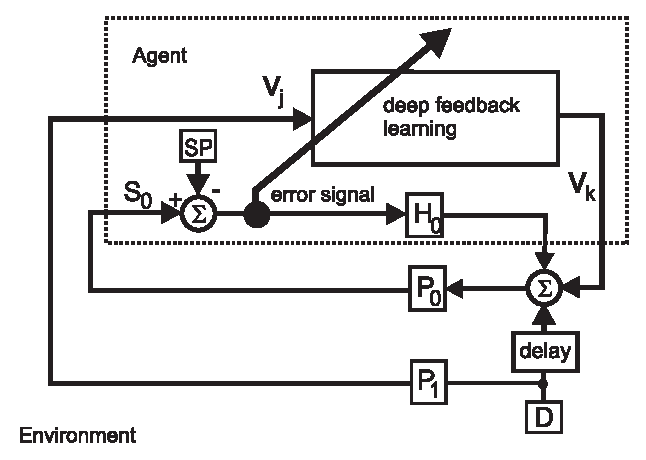
\includegraphics[width=0.75\columnwidth]{closed_loop}
  \caption{A closed loop system with a setpoint $SP$, transfer
    function $H_0$ and the environment $P_0$ which needs to work
    against unpredictable disturbances $D$.  The error signal tunes a
    deep neuronal network, which has inputs $V_i$ that predict the
    disturbances. The network tries to pre-empt these disturbances and
    generate an appropriate action $V_k$. The transfer functions here
    are indicated with capital letters and are in the sampled
    z-domain.
    \label{closed_loop}}
\end{figure}

\section{Closed loop learning}
Before we describe the algorithm, we need to place it in a simple and
instructional closed loop context. Fig.~\ref{closed_loop} shows the
entire closed loop system, with the deep feedback learning as a black
box for now. The idea is that we have a fixed closed loop which is
able to fend off disturbances, such as an unexpected bend on a road or
the sudden appearance of an enemy. This fixed loop then takes
appropriate action to solve this disturbance, e.g. correcting a car's
steering, targeting food or aiming towards and shooting an enemy.

In formal terms we have a setpoint $SP$ which compares the input of an
agent to a desired input. If the input deviates from the setpoint an
action is generated with the transfer function $H_0$ which turns the
sensor input into an appropriate action. This action then eliminates
the disturbance $D$ and arrives via the environmental transfer
function $P_0$ back at the input again; thus, the loop is closed. Such
a system is called a reactive system or ``reflex'' since it reacts
after a disturbance has occurred. Such a reaction is rigid and
designed in a way that it can deal with the disturbances
encountered. In biology this is often called ``reflex'' as it reacts
in a stereotypical way but guarantees that the closed loop
operates. For example when we trip over a fast reflex generates a
quick reaction to restore a normal walking gait as quickly as
possible. The reason why we have chosen a feedback loop because it
generates a simple but instructive \textsl{error signal}. The error
signal is non-zero if a disturbance has happened, and this can be used
to tune our deep feedback learning network.

In order to tune our network it receives additional inputs which are
able to predict the disturbance, and thus prevent the trigger of the
feedback loop via $H_0$ and $P_0$. These additional inputs are
provided via $V_i$ where we have shown one pathway and possible
additional inputs as a dashed line in Fig~.\ref{closed_loop}). For
example a video camera or eyes can provide images of the way ahead, or
of an enemy prior to attacking. Our algorithm has the task of using
the error signal to tune its network and to minimise this error, as
described next.

\begin{figure}[!ht]
  \centering
  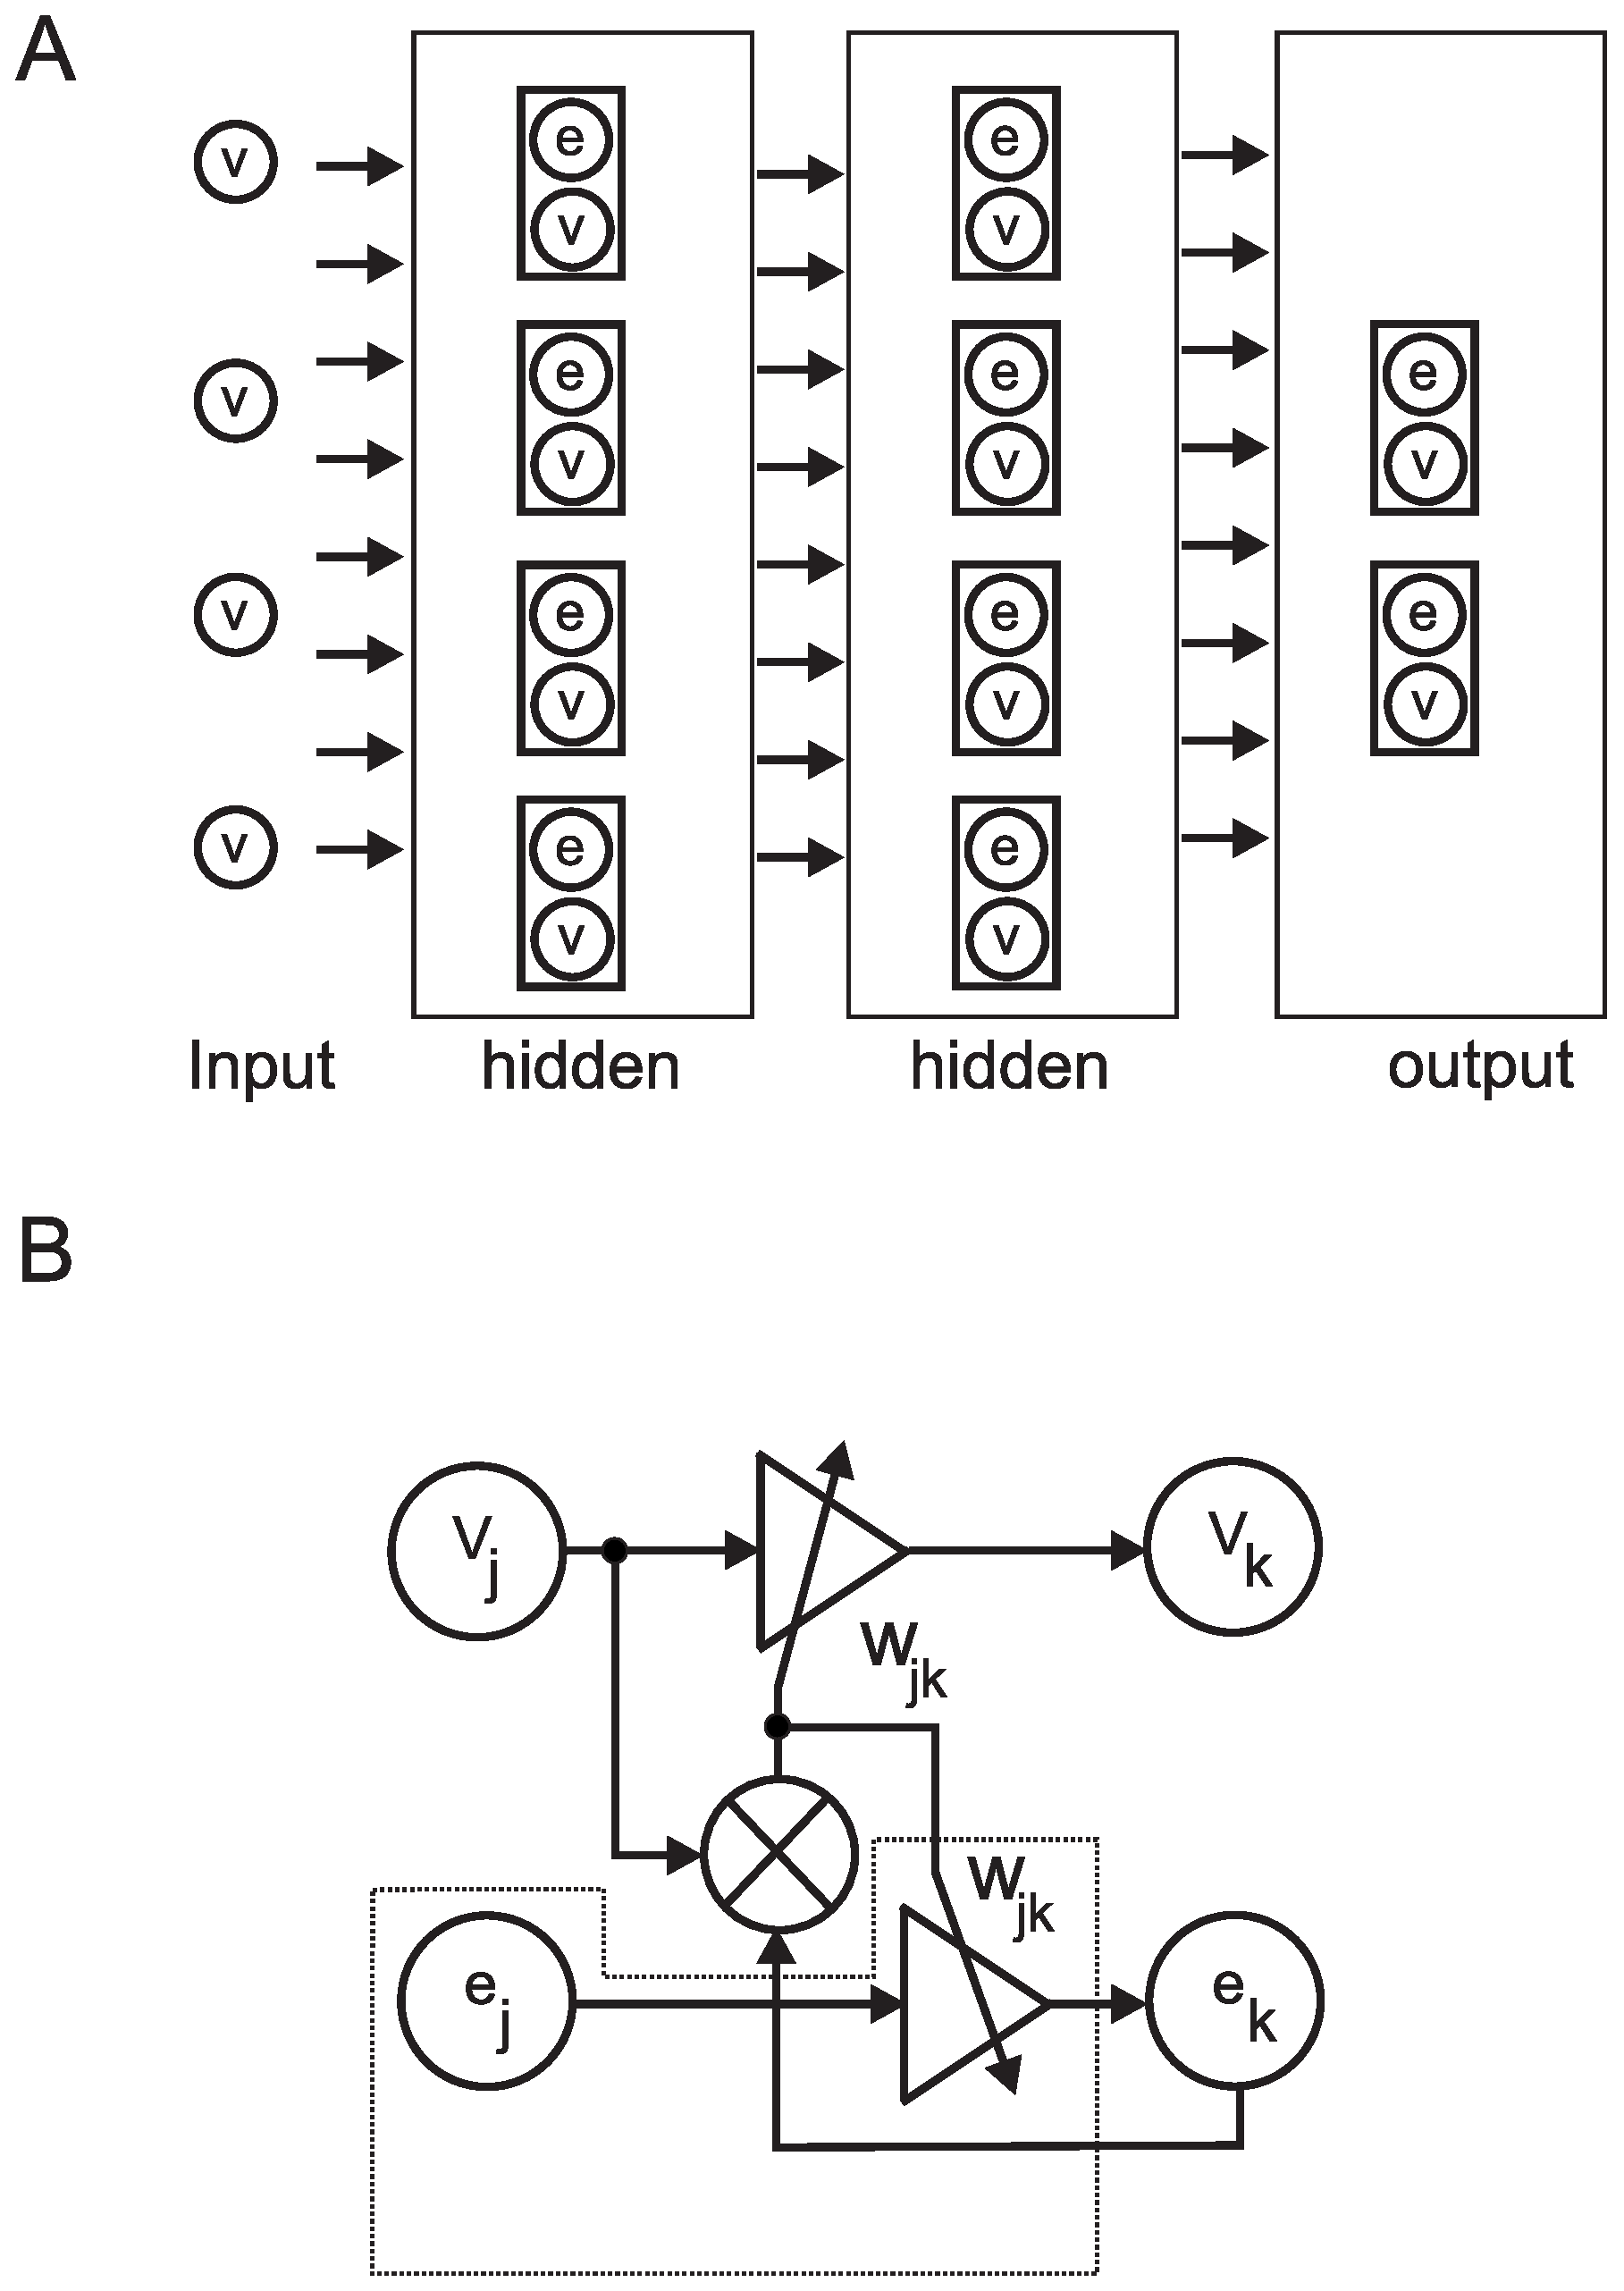
\includegraphics[width=\columnwidth]{netw_together}
  \caption{A) Network overview. With the exception of the input layer, every
    neuron is a composite cell with an activation $v$ and an error
    term $e$. These are propagated through the network in a weighted
    fashion in parallel.  B) Computation in a single composite cell.
    The presynaptic activities $v_j$ and error signals $e_j$ are used
    to perform correlation based learning and change the weight
    $w_{jk}$ which weights for both activity and error propagation into the next
    layer. The contents of the dotted box only exist for the deeper
    layers as also illustrated on the left with the input layer
    having only activities $v$, but no errors. \label{netw_together}}
\end{figure}

\section{Forward Propagation Closed Loop Learning}
We define a network with an input layer, hidden layers and an output
layer, which can all have different numbers of neurons (see
Fig~\ref{netw_together}A). In contrast to traditional
networks, every layer (except for the input layer) consists of two
summation nodes: the actual activity and an error signal. These
are processed in two parallel streams.

Let us first focus on the network activity. We define a multi-layered
network, where every neuron in any layer is a standard computational unit that
calculates a weighted sum $v_k$ of its inputs $v_j$ and then applies
an activation function $\Theta(x) = \tanh(x)$:
\begin{equation}
  v_k = \Theta\left( \sum_j w_{jk} v_{j} \right) \label{act_sum}
\end{equation}
The activity flows from neurons in layer $v_j$ to neurons in
layer $v_k$ multiplied by the weights $w_{jk}$, and this
is then repeated in the next layer. For a network with
$N$ layers we have then $N-1$ sets of weights $w_{jk}$. Note that these
indices are just examples and we start with $i$ for the 1st layer and then
$j$ and so on.

The weight changes are then updated in a semi-Hebbian fashion:
\begin{equation}
  w_{jk}(t+1) = w_{jk}(t) + \gamma v_j(t)  e_k(t) + \mu \Delta w_{jk}(t) \label{learningRule}
\end{equation}
where $v_j(t)$ is the presynaptic activity and $e_k(t)$ is an error
signal attached to the postsynaptic neuron, so the correlation is
calculated between input signals and the error signal, with the
standard parameters learning rate $\gamma$ and momentum $\mu$.

We now describe the error signal propagation. As outlined above, the
error signal emerges from the feedback loop, and is injected into the
network at the 1st hidden layer as the ``postsynaptic'' activity. The
weight change for this 1st layer can then be calculated directly with
Eq.~\ref{learningRule} by setting $e_k$ to the error signal of the
feedback loop (see Fig.~\ref{closed_loop}).

For the deeper layers, the error signal is computed as a weighted
sum of the error signals from the previous layer:
\begin{equation}
  e_k = \frac{\left( \sum_j w_{jk} e_{j} \right) \Theta^\prime (v_k) }{\frac{\sum_j {|w_{jk}|}}{\sum_j 1}}
  \label{deepError}
\end{equation}
where the $\Theta^\prime (v) = 1 - v^2$ is the derivative of the
activation function $\Theta(v)$: this limits learning when the unit
approaches saturation, as in backprop. The norm guarantees that
the error propagates through all layers and does not vanish from
layer to layer due to small weights.

In order to have an intuition about this novel learning approach we
have drawn one of the learning units establishing a layer which is
shown in Fig~\ref{netw_together}B, where we see the two processing
streams: both the activity $v_j$ and error signal $e_j$ are weighted
by $w_{jk}$, and summed separately in the next layer with index $k$.
Remember that for the 1st hidden layer, the error is just the error
signal directly injected from the feedback loop which then equates to
$e_j$. Then the next layer receives the weighted errors $e_k$ and
activations $v_k$. The diagram omits the error normalisation, scaling
and activation derivative in order to focus on the main point that
learning happens between the error signal and the presynaptic activity
and that both error signal and activation are transmitted in a
weighted fashion.

Learning is therefore performed in three steps: first the activity is
propagated through the network, then the error signal is propagated
via the \textsl{same} weights, and finally the weights are adjusted. Thus,
both the error signal and the activity are propagated in a forward
fashion. Learning itself can be interpreted as \textsl{heterosynaptic} for the
activity $v_j$ and \textsl{Hebbian} for the error $e_j$.


\section{Derivation of the learning rule}
We start from the assumption that a single neuron using heterosynaptic
plasticity is able to eliminate a closed loop error signal
\cite{Porr2006ICO}. Because of the exploding complexity of closed loop
learning we focus here on how an error signal $X_0$ should be propagated
to deeper layers from its input by using the approach in
\cite{Mehta1986}, taking partial derivatives in the z-space and
assuming that weight development in time is slow in comparison to the
closed loop dynamics.  Let us assume two layers $j$ and $k$ where the
input signals to the deep network are signals with index i so that we
have $V_i, V_j$ and $V_k$. The error signal, $X_0$ (see
Fig.~\ref{closed_loop}), can be expressed as
\begin{equation}
  X_0 = \frac{P_0 \left[ V_k V_J + D z^{-1} \right]}{1-P_0 H_0}
\end{equation}
where $V_k$ and $V_j$ are transfer functions of the layers $k$ and $j$
respectively. We know that a weight change $\Delta w$ calculated by
correlating $X_0$ with an input $V_i$ leads to convergence in a closed
loop system \cite{Porr2006ICO}. This can be expressed as:
\begin{equation}
  \Delta w_{ij} = X_0(z) V_i(-z)
\end{equation}
which is the correlation between the error signal $X_0$ and the
signal $V_i$ in the sampled z-space.

We now need to show that if we have deeper weights such as $w_{jk}$
that these will change in the same way as those of the input layer. In
order to establish this, we look at small weight changes in $w_{jk}$
and relate them to the input weights $w_{ij}$.
\begin{equation}
    \frac{\partial X_0}{\partial w_{jk}} =
    \frac{\partial X_0}{\partial V_j}
    \frac{\partial V_j}{\partial V_k}
    \frac{\partial V_k}{\partial w_{jk}}
\end{equation}    
where
\begin{equation}
\frac{\partial X_0}{\partial V_j} = \frac{P_0 V_k}{1-P_0 H_0}
\end{equation}
If we assume for now that the layers consist only of linear neurons:
\begin{eqnarray}
  V_k &=& \sum_j w_{jk} V_j \\
  V_j &=& \sum_i w_{ij} V_i
\end{eqnarray}
then this yields:
\begin{eqnarray}
    \frac{\partial X_0}{\partial w_{jk}} &=&
    \frac{P_0 V_k}{1-P_0 H_0}
    \frac{\partial V_j}{\partial V_k}
    V_j \\
                                        &=&
    \frac{P_0 V_k}{1-P_0 H_0}
    \frac{\partial V_j}{\partial V_k}
    \sum_i w_{ij} V_i
\end{eqnarray}    
  We can now multiply this equation with $V_i(-z)=V_j^-$ to indicate a correlation, yielding:
\begin{equation}
    \frac{\partial X_0}{\partial w_{jk}} V_i^- =   
    \frac{P_0 V_k}{1-P_0 H_0}
    \frac{\partial V_j}{\partial V_k}
    \underbrace{\left( \sum_{i^\prime} w_{i^\prime j} V_{i^\prime} \right)}_\textrm{\tiny deep layer error signal} V_i^-
\end{equation}
This means that if we introduce a small change in the deeper weights
$w_{jk}$ they will depend on the weighted covariance at the input
where this correlation at the input propagates, weighted by the input
weights $w_{ij}$, to the deeper layer $w_{jk}$. This shows that the
error signal is propagated in a weighted fashion to deeper
layers. Note that this is not a stability proof but rather the
derivation of the network structure, using a similar trick to deep
learning but in closed loop and forward fashion. For a stability
analysis one needs to take into account for the non-linear activation
functions and unroll the partial derivative $\frac{\partial
  V_j}{\partial V_k}$, whose derivative depends again on the entire
closed loop. However, this is not of practical relevance because the
environmental transfer function is rarely known; this leads us to
the shooter game.



\begin{figure}[!ht]
  \centering
  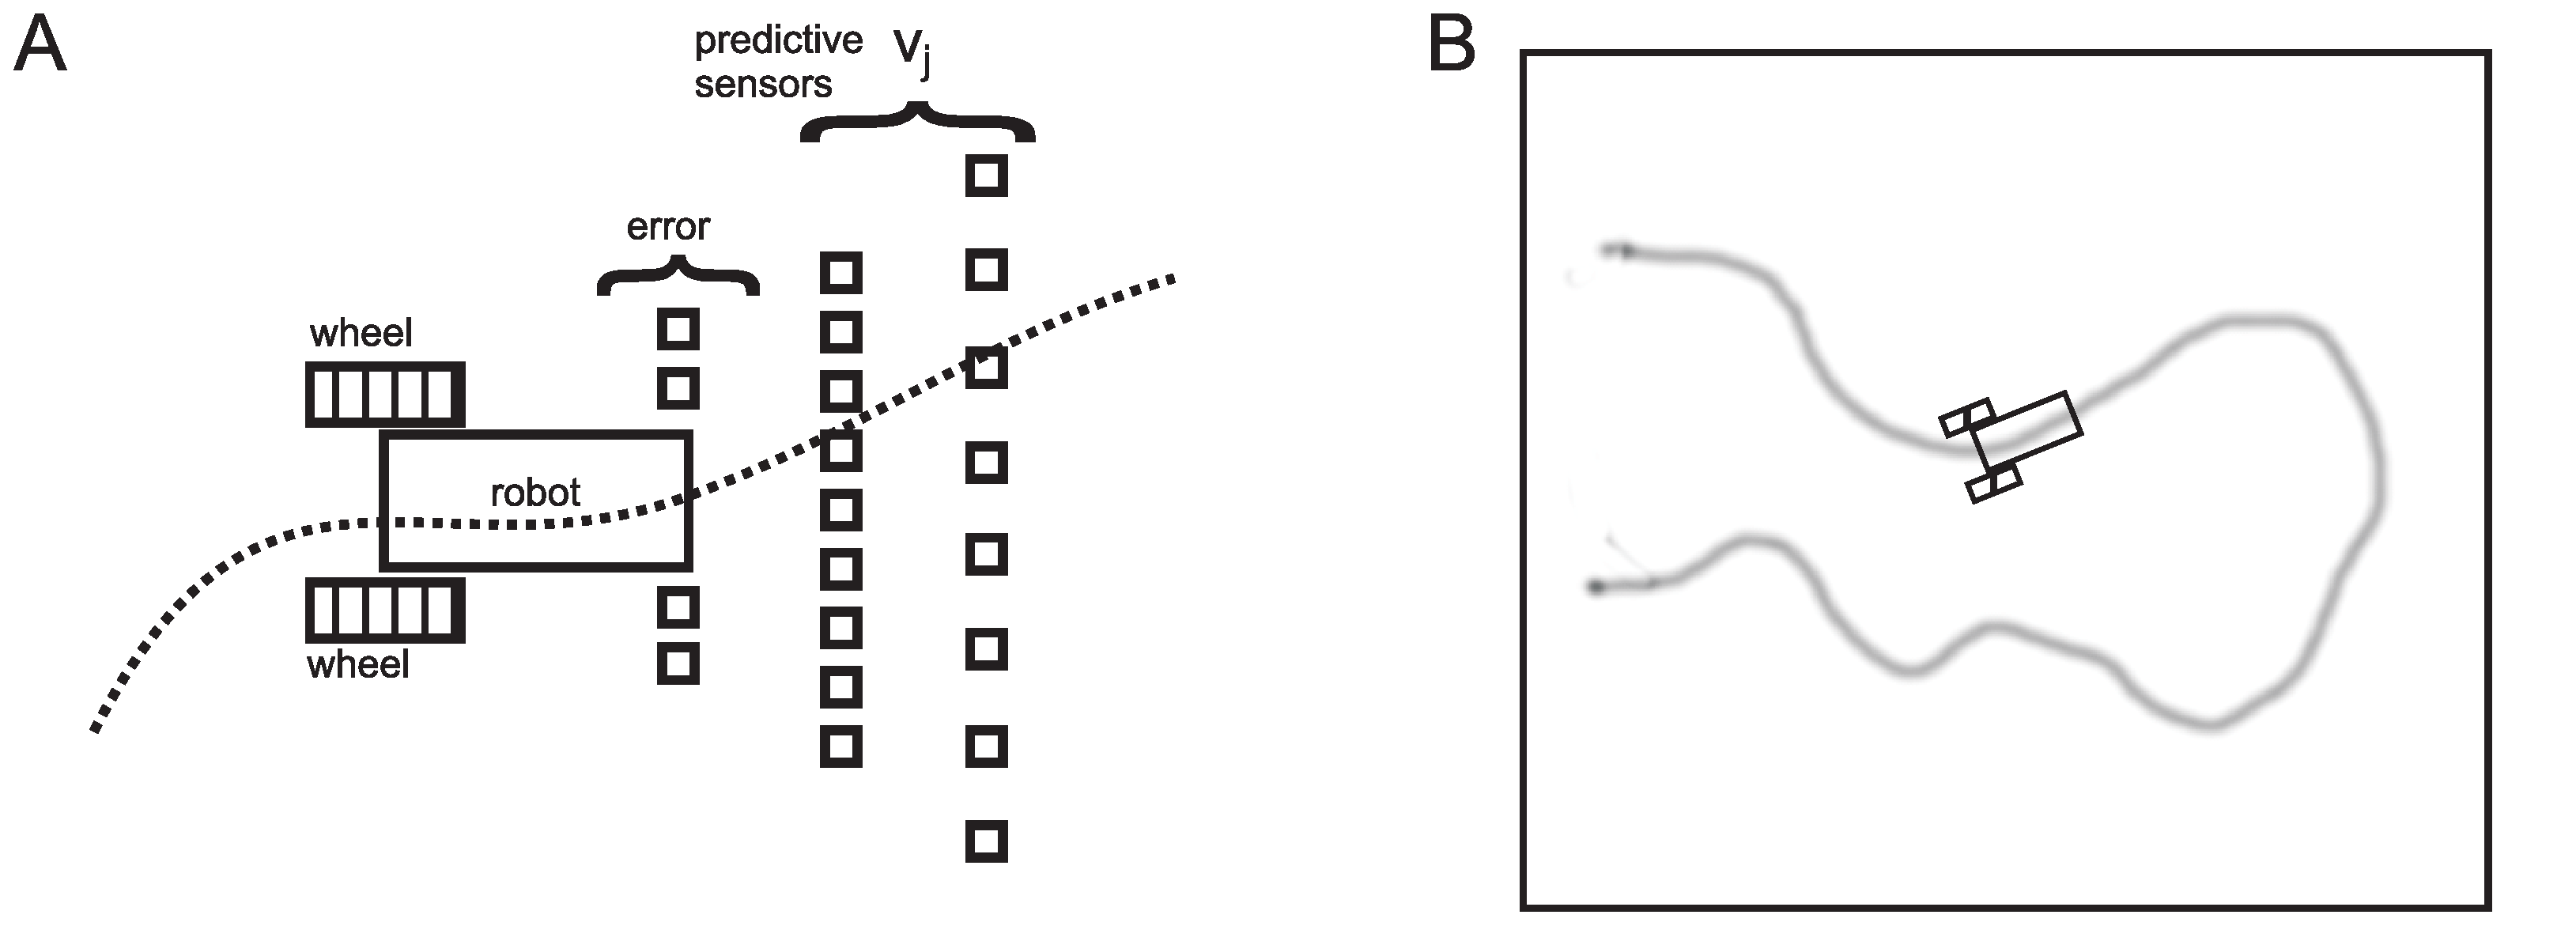
\includegraphics[width=0.85\columnwidth]{linefollower_robot_playground}
  \caption{A) Robot setup. The robot is simulated with a updated
    version of enki for QT5 (\texttt{https://github.com/glasgowneuro/enki})
    where the line follower is using just the ground sensors of the
    robot to create the error signal ($g_l$, $g_r$) and the predictive signals ($p_m$)
    for FCL. Each of the 30 predictive signals $p_m$ from the two rows of ground sensors
    is split into 10 2nd-order lowpass filters with impulse responses
    lasting from $2$ to $30$ timesteps, and then these all feed into the FCL
    network as predictive inputs $v_j$, giving 300 inputs in total.
    The robot has two wheels whose speed is controlled
    by the feedback control and FCL.
    B) The line following scenario used for the simulations. The robot
    attempts to drive along the line and is reversed at the end of the
    line and then drives back. If it hits the boundaries of the playground
    it is also turned around.
    \label{linefollower_robot_playground}}
\end{figure}

\begin{figure*}[!ht]
  \centering
  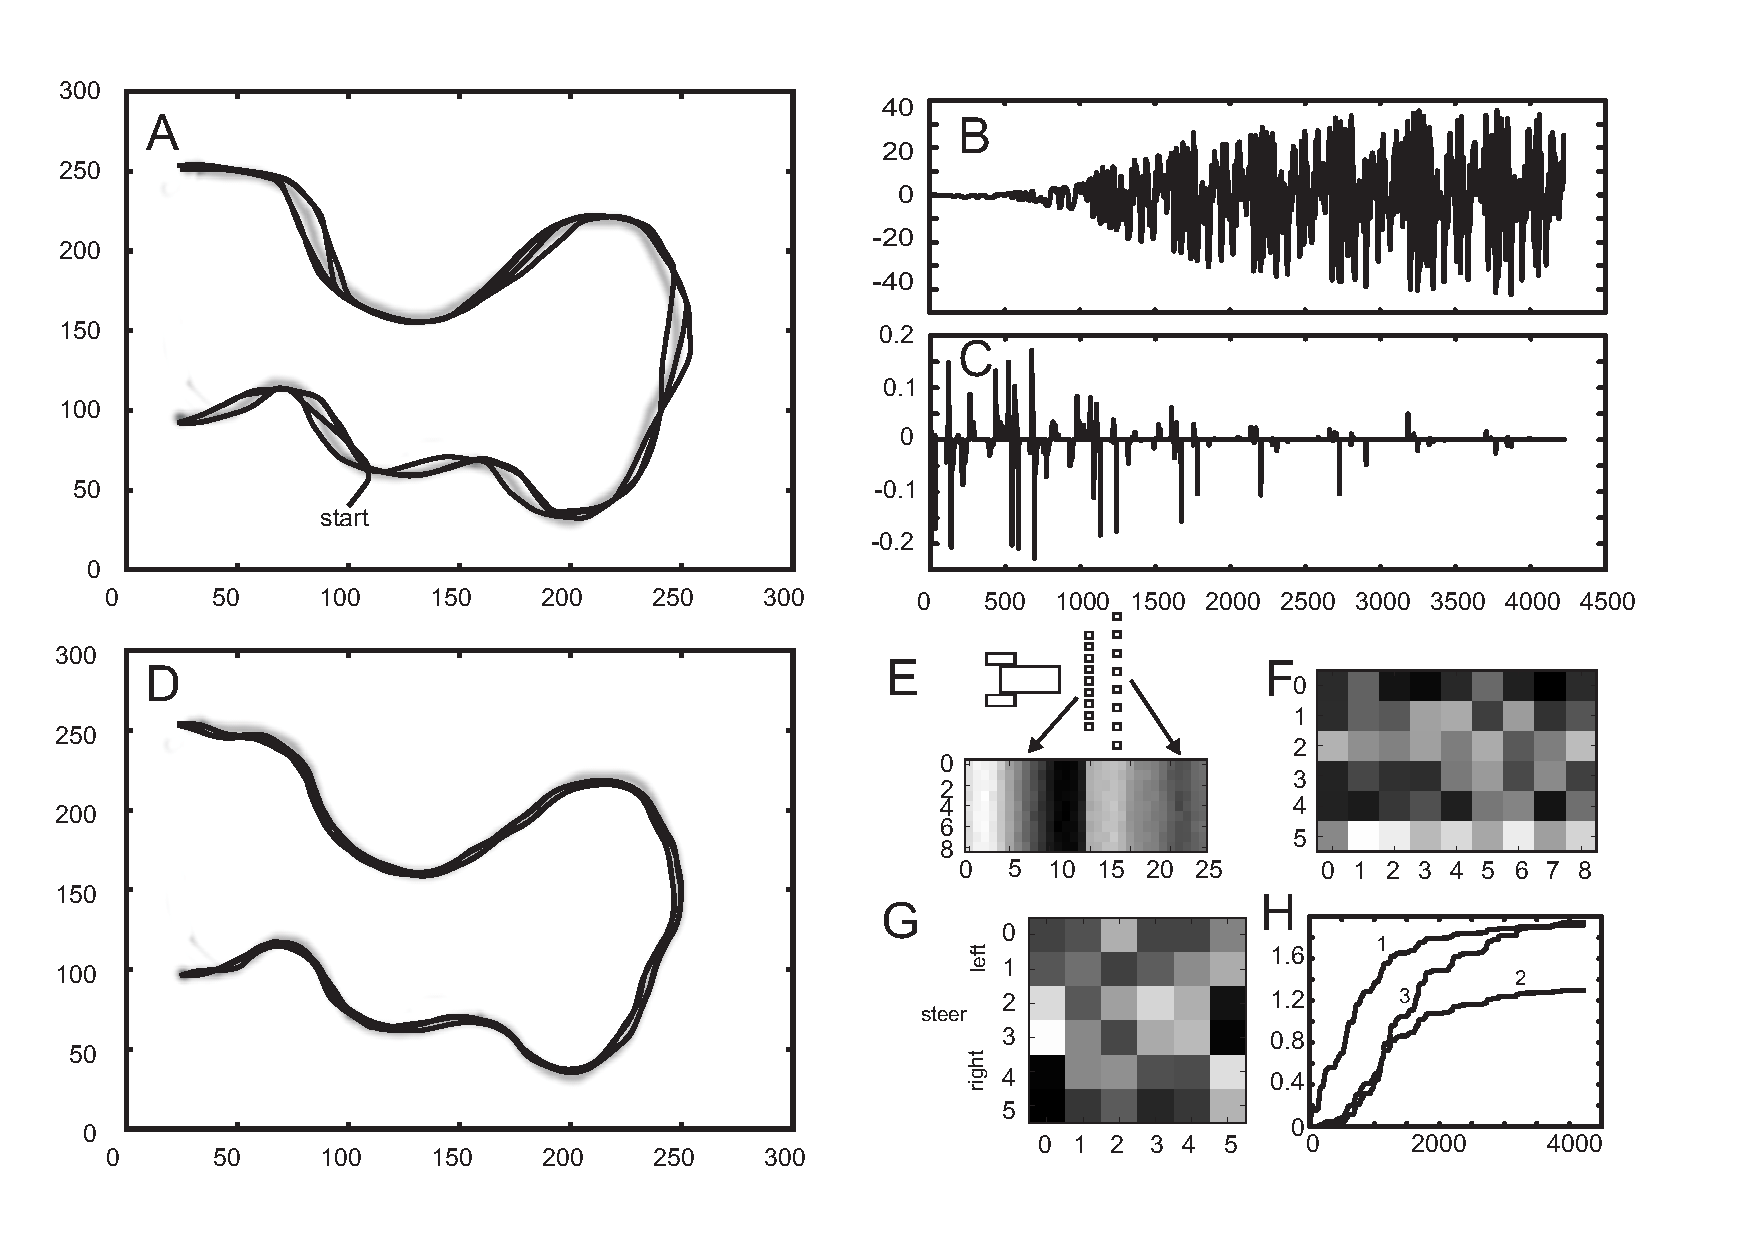
\includegraphics[width=\linewidth]{line_results}
  \caption{Results of the line following task. A) shows the robot at
    the very start of the simulation run from time step 0 to 1000. B)
    the difference between the robot wheel speeds just for the learned
    actions (i.e. the output of the FCL network): $v_l-v_r$.  C) the
    error signal.  D) simulation run just before the final 1000 time
    steps where the absolute value of the error has been below 0.001
    for 1000 time steps. E-G) show the weights of the different
    layers. The input neurons are on the x-axis and the output neurons
    are on the y-axis.  E) the weights of the 1st layer, F) the
    weights of the 2nd layer and G) the weights of the output layer.
    H) shows the euclidean distance of the weights for each layer from
    their random work initialisation. Parameters: 30 inputs from two
    predictive rows of sensors (15 each). Every input was fed into a
    filterbank of 10 filters with T=2 \ldots 30. There were 2 hidden
    layers with 9 and 6 neurons; 6 output neurons. The learning rate $\gamma$
    was 0.0001 and the momentum $\mu$ was set to 0.9. Learning was disabled
    when the robot turned to avoid large error spikes caused by the learning
    and the error was also set to zero during turning.
    \label{line_results}}
\end{figure*}








\section{Line follower}
In order to demonstrate and benchmark FCL we need a simple closed loop scenario
which can be improved with the help of an adaptive network.
Fig.~\ref{linefollower_robot_playground} shows a simple line following
robot which has the task of following the line depicted in
Fig.~\ref{linefollower_robot_playground}B to the end, where it
reverses and drives back, and so on. The four ground sensors in
Fig.~\ref{linefollower_robot_playground}A left/right on either side
of the robot create an error signal:
\begin{equation}
\mathrm{error} = (g_{l_1}+2 g_{l_2})-(g_{r_1}+2 g_{r_2}) \label{line_error}
\end{equation}
this error directly creates a steering reaction from the fixed
feedback loop by controlling the speed of the wheels.

The FCL learning circuit uses the predictive ground sensors - these
are first filtered by a filterbank, which smears them in time and
creates a temporal overlap with the error signal. These filtered
signals are then presented to the $v_j$ of the input layer (see
Eq.~\ref{act_sum}). We have two rows of sensors, one directly in front
of the robot and one which looks further ahead. There are 30 ground
sensors each filtered by 10 filters, giving 300 inputs in total.

The output layer of our feedback learner consists of 6 neurons
with activations $v_k$ ($k=0 \ldots 5$) - these can be seen as soft
decision-making units where 3 of them determine the change of speed of
the right wheel, and 3 the left wheel. This leads to the
final formulas for the motor outputs:
\begin{eqnarray}
  \mathrm{leftSpeed} &=& s_0 + \underbrace{g\, \mathrm{error} + \left( 50 v_0 + 10 v_1 + 2 v_2 \right)}_{v_l} \\
  \mathrm{rightSpeed} &=& s_0 - \underbrace{g\, \mathrm{error} + \left( 50 v_3 + 10 v_4 + 2 v_5 \right)}_{v_r}
\end{eqnarray}
where $v_0, \ldots, v_5$ are the 6 outputs from the FCL network. Note
that neither inputs nor outputs are organised in a topographically
meaningful way. The network must discover from the error signals
which sensor inputs $v_k$ will eventually lead to appropriate steering
actions. At the start the network is initialised with random values.

As performance criterion we use the absolute value of the error from
Eq.~\ref{line_error}:
\begin{equation}
  \mathrm{error}_\mathrm{abs} =  |\mathrm{error}| \label{line_abserr}
\end{equation}
which needs to be below a threshold of $0.001$ for 1000 time steps
because realistically, driving will never be 100\% perfect, and we
allow $\mathrm{error}$ to stabilise at small values.


\subsection{Results}
Fig.~\ref{line_results} shows the results of a simulation run. In the
panels A) and D) we see the trajectory of the agent over the course of
4225 time steps of learning. While in A) the agent clearly just
follows the reflex reaction, leading to large deviations from the
track, in D) the agent closely follows the track and the deviation is
minimal -- learning has been successful. In B) we see the network
learning to generate steering actions that keep the agent closely on track.
It can be seen that the network clearly slows down in the change of
output.  C) shows the error quickly dropping to near zero, leaving
only small components remaining. E) is the final weight matrix of the
1st layer after learning, which correlates the error with the two rows
of predictive ground sensors $v_j$. F) is the weight matrix of the
hidden layer and G) of the output layer. H) shows the Euclidean
distance of the different layers from their starting point.

Overall, Fig~\ref{line_results} shows that the network learns to use
the predictive signals from the sensors in front of the robot to
generate its steering output. This steering output slowly becomes
stronger and then stabilises.

The error in Fig.~\ref{line_results}C slowly decays
leaving only small spikes remaining which eventually vanish. Even
if small errors remain, as long as they average out the weights
will stabilise.

The weights of the various layers are shown in
Fig.~\ref{line_results}E-G. The weights in the input layer
(Fig.~\ref{line_results}E) show a slow gradation from left to right as
expected. Recall that there are two rows of predictive ground
sensors in front of the robot; these cause two different weight maps
which can clearly be seen. The inputs 0 to 14 correspond to the near
ground sensor, and 15 to 31 the far sensor which looks further ahead, 
helping the robot predict bends better. These feed then into the 
hidden layer Fig.~\ref{line_results}F
and from there into the output layer Fig.~\ref{line_results}G.

The overall weight development per layer over the time is shown in
Fig.~\ref{line_results}H. Recall that the error signal is weighted by
the weights for the deeper layers, but also normalised, so therefore
learning happens at approximately the same rate in every
layer. However, the deeper layers show more of an exponential
growth. One might think that his is because learning uses both
cross and autocorrelation, but even removing the autocorrelation
term in Eq.~\ref{deepError} does not change the development, which implies
that the environmental feedback is responsible for this development.

\begin{figure}[!ht]
  \centering
  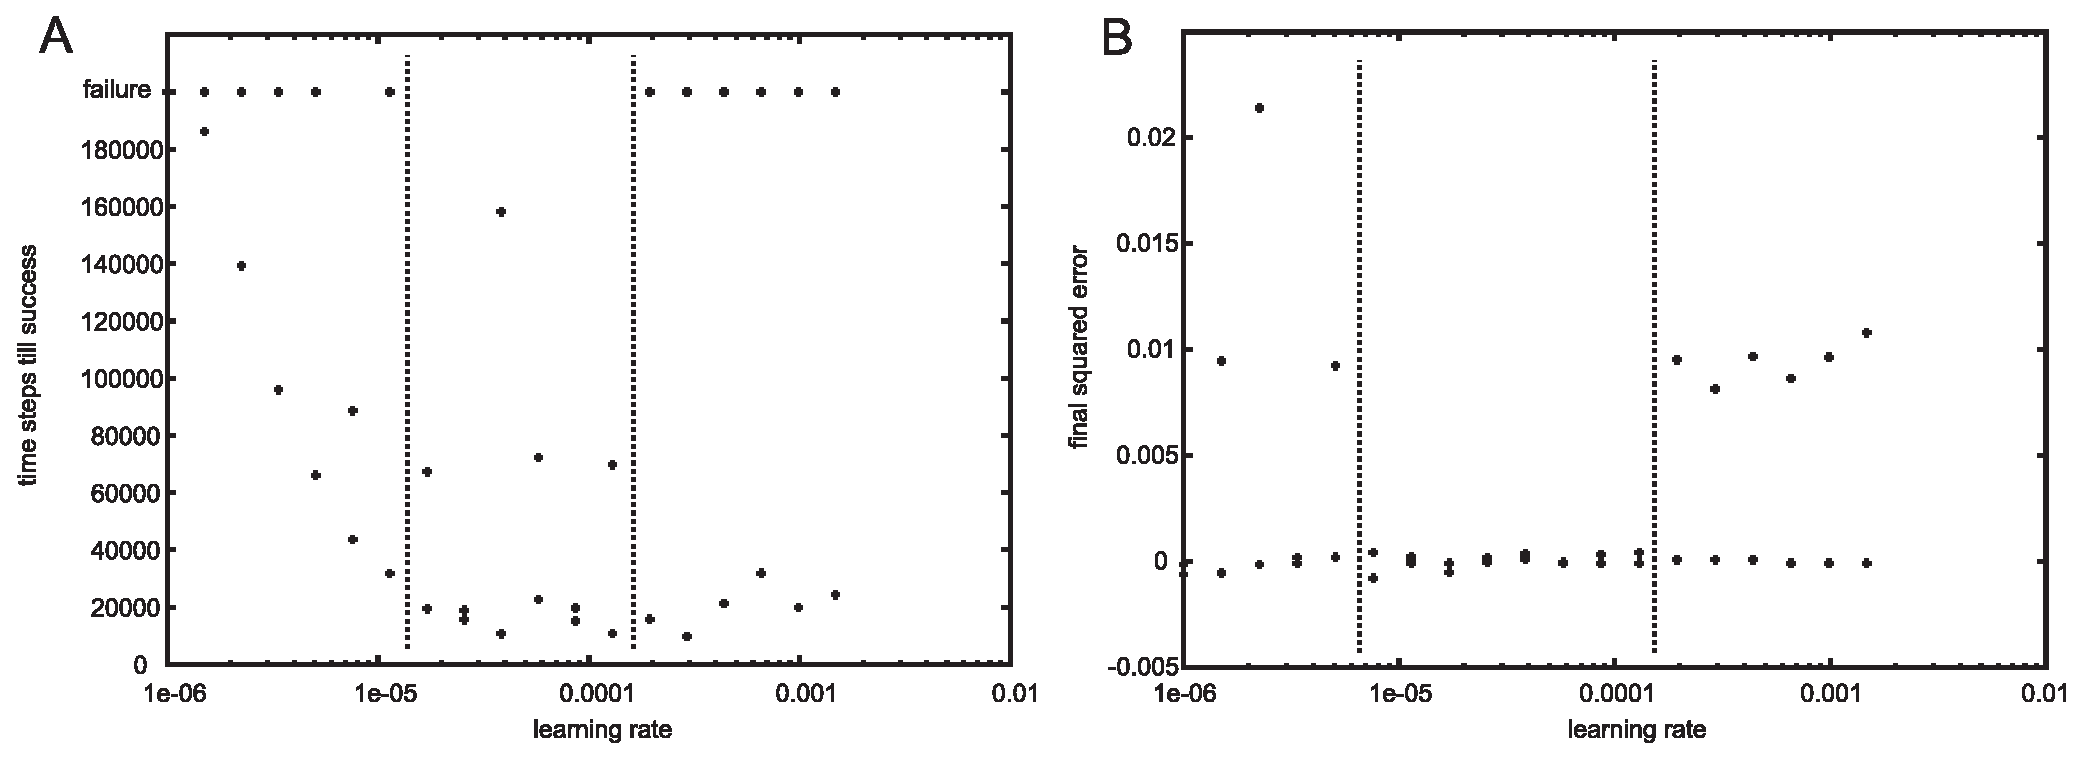
\includegraphics[width=0.9\columnwidth]{line_stats}
  \caption{Statistics of the line following task. A) shows the relation between
    'time to success' and learning rate. For every learning rate two runs have
    been conducted with different random number seeds to test the dependence on the
    initialisation of the weights. The simulation was marked successful if the
    absolute value of the error Eq.~\ref{line_abserr} stayed below $0.001$ for more than $1000$
    timesteps. The simulation was aborted after $200,000$ time steps if this criterion
    hasn't been reached. Inside of the square every run has been successful.
    B) shows the final absolute error for different learning rates.
    \label{line_stats}}
\end{figure}


We have run statistics of the line follower where we varied the
learning rate over three orders of magnitudes, and evaluated how long
it takes to stay below the error threshold for a specified time
(Fig.~\ref{line_stats}A), and the resulting absolute value of the
error (Fig.~\ref{line_stats}B). The time to reach the criterion
decreases with higher learning rates, and is stable up to a learning
rate of approx $\gamma = 0.001$ with no failures below a learning rate of
$\gamma = 0.0002$. Each simulation was run twice with two different random seeds to
test for initialisation effects -- it can clearly be seen that
the seed has an effect on both the number of simulation steps,
and at higher learning rates the final error, which is in agreement with other neural
network architectures that initialisation matters.


\section{Shooter game}
In this scenario, we try to learn to play a first-person shooter
purely from visual inputs. We use the Vizdoom
(http://vizdoom.cs.put.edu.pl/) environment for this purpose, and
train a controller to play against a single pretrained bot from Intel
that ran in the Vizdoom 2016 competition. The setup was as follows:

The images returned from Vizdoom are RGB 160x120. We rendered the
enemy in blue, and formed a reflex signal by finding the bounding box
of the pixels closest to that colour. Note that the reflex is slow and
also inherently noisy, as other events in the game are also rendered
blue (e.g. the ‘flashes’ that happen at respawns). The reflex also
fails at times when the enemy is too distant or too close to the
camera. For learning, we only supply the network with the greyscale
image (Fig.~\ref{shooter_results}D) flattened into a vector of $19200$
inputs, so it is forced to discover purely spatial cues. The reflex is
computed relative to the image centre, so a negative value implies the
enemy is on the left. Shooting behaviour is entirely hardwired: if an
enemy is detected within a threshold of the image centre, the bot
fires. Note that the bot's only actions are to rotate in the plane,
and shoot -- it does not translate (but the enemy does). To generate
the rotation we have a single value produced by 3 neurons acting at
different sensitivities:
\begin{equation}
\Delta \theta = g_{err}\, \mathrm{error} + g_{net} \left( 10 v_0 + 3 v_1 + v_2 \right)
\end{equation}
where $v_0, \ldots, v_2$ are the network outputs, and $\Delta \theta$
is the change in orientation. The three output neurons have $tanh$ activation; a
negative output means ‘rotate left’, a positive ‘rotate right’. The 3
neurons operate with different gains, to give finer control. The terms
$g_{net}$ and $g_{err}$ are the gains for the reflex, and the learned
control signal. Momentum was 0.5; weights were initialised in a zero-mean
uniform distribution, scaled by the number of weights outputting each
neuron.

\begin{figure*}[!ht]
	\centering 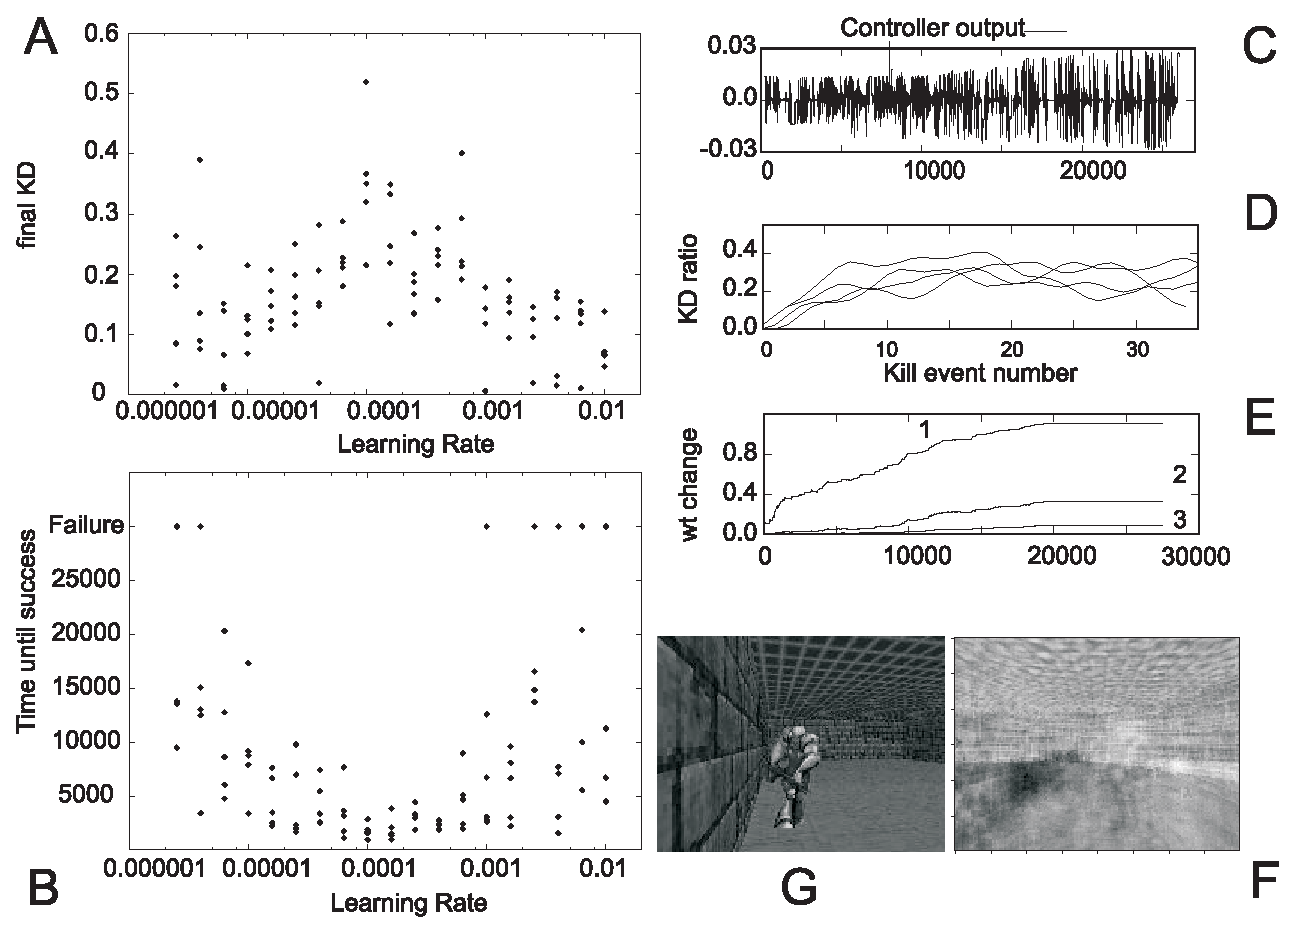
\includegraphics[width=\textwidth]{FPSFig7}
	\caption{A) KD at end of trial. B) Time to success vs learning
          rate - success is if the smoothed KD ratio reaches a
          threshold of 0.15. C) Example input frame. D) Example input weights.
          E) $\Delta \theta$, the rate of change in
          bot's orientation against simulation step number, purely
          from the learned FCL output, in arbitrary units. F) KD learning
          curves - the time series of kills/deaths is filtered with a
          2nd order lowpass filter to get a moving average, plotted
          against kill event number. G) Euclidean distance of weights
          for each layer from their initial point, against learning
          step.
          Parameters: 19200 inputs from grayscale image; 2
          hidden layers of 5 units each. Inputs were
          normalised to zero-mean, unit variance. Learning rate in E, F
          and G was 0.0001.
		\label{shooter_results}}
\end{figure*}

\subsection{Results}
It can be clearly seen that the controller outputs steadily increase over
time (Fig.~\ref{shooter_results}E). With a high value of $g_{net}$,
the bot can make very rapid aiming movements. This has the advantage
that the error can in principle be reduced very quickly; it also
causes the bot to sometimes make large rotations even when the enemy
is out of the field of view, which helps with exploration. On the
other hand, it can cause the aiming to overshoot and oscillate around
the target. The weight growth is intermittent due to the discontinuous
nature of the error signal (Fig.~\ref{shooter_results}G) but stabilises
because the long term average error converges to zero. The different
scales are likely due to the inputs having more dimensions.

A popular performance measure in gaming is how often the bot is killed
vs how often it kills the enemy. This is called the kill/death ratio,
and we plot some smoothed KD curves in Fig.~\ref{shooter_results}F. To
do statistics, we measure the time taken to reach a threshold KD of
0.15 - Fig.~\ref{shooter_results}B shows this as a function of
learning rate. There is a stable region in the middle where
learning is consistently successful. We also plot the smoothed KD for
the final step of each trial(Fig.~\ref{shooter_results}A); although a
noisy measure, the same pattern emerges. Over time, the input weights
blur the background, leaving dark and light blobs to detect the enemy
and generate an aiming response (Fig.~\ref{shooter_results}D).

Note that this is only one skill of a functioning FPS bot, as a real
bot would require additional skills such as seeking rewards
(e.g. finding health packs) and navigating the environment
(e.g. avoiding collisions). Future research will investigate whether
the FCL approach can be used to acquire such skills, for example,
by utilising the reward prediction error generated by TD learning.


\section{Discussion}
We have shown that a network which propagates its errors in a
forward fashion from its inputs to its outputs is able to solve closed
loop learning tasks. We have demonstrated this in a first person
shooter game and with a simple line follower.

Plasticity has always been hotly debated in neurophysiology -- the
general understanding is that a large postsynaptic Calcium
concentration causes LTP \cite{Malenka99,Bennett2000} and a low one
causes LTD \cite{Mulkey1992}. This requires a strong presynaptic drive
to achieve a strong postsynaptic activity, and with that Calcium
influx \cite{Meunier2017}. In mathematical terms this would just lead
to self-amplification of the synaptic weight, where strong presynaptic
activity would cause greater postsynaptic activity and in turn
stronger weights, and so on. However, suppose the learning signal and
the actual activity were transmitted via the same synapse but were
fundamentally separated \cite{Lindsay2017}, for example by using
different frequencies: high frequency potentials could cause
plasticity changes via high frequency potentiation (HFP) while low
frequency potentials propagate behaviourally-relevant activity
\cite{Canolty2010}. FCL can provide here a mechanism that allows
stable behaviourally-relevant learning driven by heterosynaptic
plasticity and Hebbian learning for the error signal, with the
stability arising from the fact that it is constantly corrected by the
error signal.

Looking at a system-wide perspective, one can see FCL as a flexible
actor which has a high degree of freedom in generating actions, as long as they
minimise the error. For example in the basal ganglia the striatum is
seen as an actor receiving an error signal via dopamine, the well known
reward prediction error \cite{Schultz97} which is understood as being
closely related to the error of temporal difference (TD) learning
\cite{gurney98:_basal_gangl_action_selec_devic}. It is curious that
the striatum receives the error signal but both downstream neurons in
the basal ganglia and upstream in the cortex receive much less
dopaminergic modulation \cite{Beckstead1979}. However, plasticity is
not just limited to the striatum, but happens in all brain areas, so
it makes sense to propagate this error signal further into the cortex
\cite{Groenewegen1993} where high level decision-making takes place.
In the language of TD learning \cite{Sutton87} this means that we
have a distributed actor where the first layer is modulated by the
reward prediction error, and then the following stages, that project
back to the cortex, use instead cross frequency coupling
as described above \cite{Lipski2017}.

Given that the error is propagated from the input to the output, the
novel aspect here is that the more layers FCL has, the more remote it
is from the immediate error feedback. This allows for increased
flexibility which is then a function of the number of layers, and
creates an actor which is far less rigid than a standard Q-learner
\cite{Dayan1992}. The actions can be substantially varied as long as
the error signal can eventually be minimised, and the variability will
be more pronounced with more hidden layers. In other words, the more
hidden layers we have, the more behavioural flexibility the agent will
show. In a biological context this means that as cortical processing
takes over in the deeper stages, it also can develop more flexibility
while still receiving \textsl{distributed} error signals rather than a
global one.

A different stance about synaptic plasticity (and ultimately how
autonomous agents learn) has been taken by the deep learning
community, which has recently claimed that error backpropagation is
biologically realistic \cite{Lillicrap2016,Roelfsema2018}. This has
been demonstrated in an abstract network with one hidden layer by
introducing a separate feedback pathway from the output of the network
to this hidden layer, but this does not take account the
cortico-striatal network mentioned above \cite{haber95}. While this
shows promising results for abstract models of biologically inspired
decision making, the implied brain connectivity is not faithful to
neurophysiological findings (see \cite{berthoud04} for an extensive
review).

While we have turned error propagation upside down to use it in a
closed loop context, \cite{Guo2014} takes a different direction, and
present an approach that still uses backprop to solve closed loop
problems. To turn the open loop backprop into a closed loop algorithm,
they embed it into Q-learning which is itself closed loop. However,
even given its major performance advances, the main drawback is the
discrete state space, which makes it hard to solve analogue problems,
and Q-learning is not biologically realistic when compared to the
biological evidence outlined above.

\bibliographystyle{SageH}

\bibliography{hebb,ours,embodiment,laplace,limbic,selbstorg}

\end{document}
